Nach dem Start der App \gls{muss} dem Spieler das Hauptmenü angezeigt werden.
Von dort aus \gls{muss} er die folgenden Optionen haben:
\begin{itemize}
    \item einen Button zum Starten eines neuen Spieldurchlaufs
    \item einen Button zum Anzeigen der \gls{Top10}
    \item einen Button zum Einsehen und Nutzen des Stores
    \item einen Button zum Einsehen der Credits
    \item einen Button zum Einsehen der Achievements\OPT{*}
\end{itemize}

Außerdem wird ein Button zur Sprachauswahl als \gls{niceToHave} betrachtet.\\

Im Folgenden werden die einzelnen Anforderungen weiter erläutert:

Der Spieler \gls{muss} in der Lage sein, den Screen zum Starten eines neuen Spiel\-durchlaufs durch den zugehörigen Button zu erreichen. Auf diesem
Screen \gls{muss} der Spieler den Spielmodus auswählen können. Dem Spieler \gls{muss} es danach möglich sein, die Schwierigkeit auszusuchen.
Nach diesen Schritten kommt der Spieler direkt auf das Spielfeld und der Spieldurchlauf beginnt.

Möchte der Spieler das Spiel pausieren, so ist dies mit einem Pause-Button möglich, welcher oben rechts auf dem Bildschirm platziert sein \gls{muss}.
Verliert der Spieler alle \gls{leben}, so \gls{muss} er einmalig die Möglichkeit haben, optional durch die Anzeige eines Werbevideos ein weiteres Leben zu erhalten und weiterzuspielen.
Ist ein Spieldurchlauf beendet und der erreichte Score ist in den \gls{Top10}, so \gls{muss} der Spieler die Möglichkeit haben, seinen Namen in Verbindung mit dem erreichten Score einzutragen.

Entscheidet sich der Spieler dazu, die derzeitigen \gls{Top10} einzusehen, so \gls{muss} er dazu in der Lage sein, diese durch einen Button im Hauptmenü aufzurufen.

Möchte der Spieler den Store besuchen und/oder neue \glspl{skin} auswählen, \gls{muss} er diesen Bereich ebenfalls von dem Hauptmenü aus erreichen können. 
Im Store \gls{muss} es dem Spieler möglich sein, aus einem von mindestens fünf \glspl{skin} für \gls{ball}, \gls{tail}, \gls{balken} und Spiel-Hintergrund auszuwählen.

Um die Credits der PONG-App einzusehen, \gls{muss} der Spieler vom Hauptmenü aus fähig sein, zu einem Credits-Screen zu gelangen. Dort findet er die Namen der Personen, die an der Entwicklung der App beteiligt waren sowie das Copyright.

Der \gls{spieler} \gls{sollte} in der Lage sein, über einen Button im Hauptmenü seine Achievements einsehenen zu können.

Figure~\ref{fig:use-case-diagram} stellt das UseCase diagramm zur App PONG dar:

\begin{figure}[h!]
    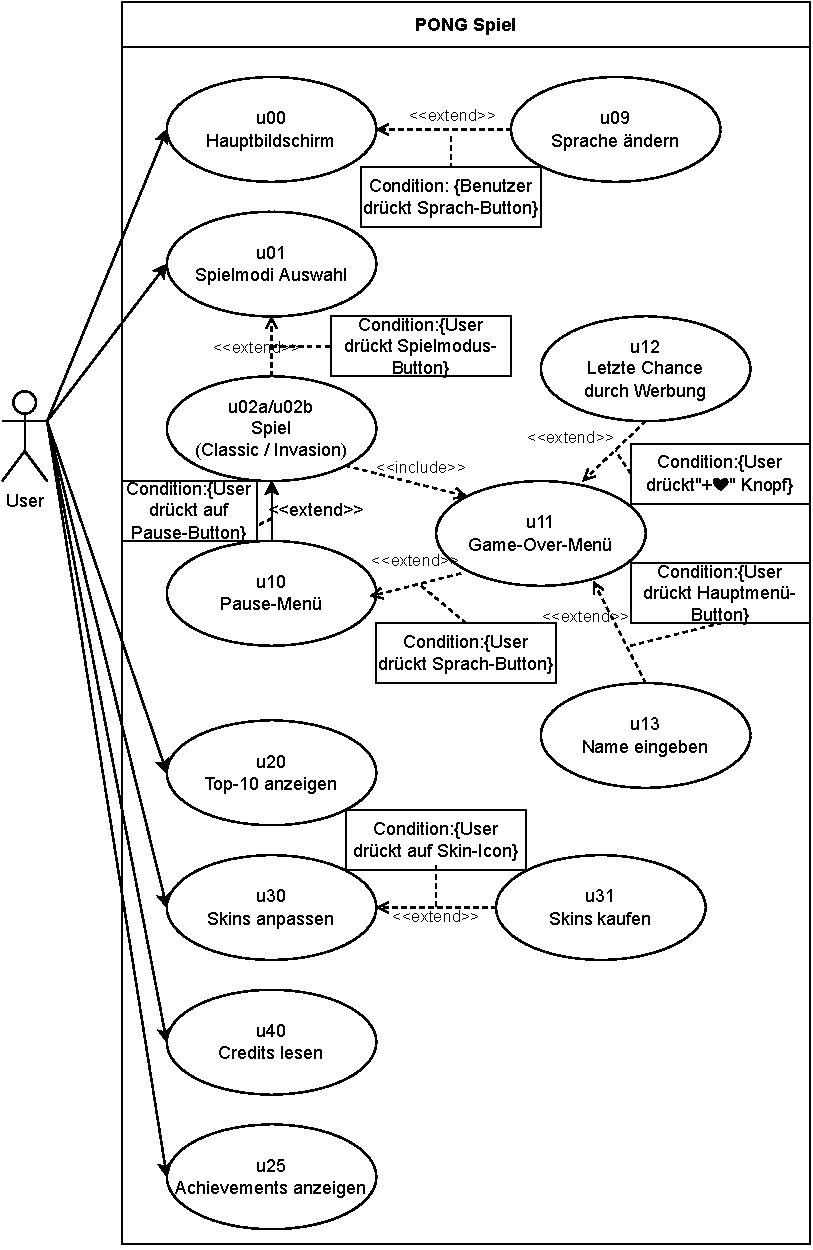
\includegraphics[width=\textwidth]{diagramme/pdf/UML-K4-UseCase.pdf}
    \caption{Use Case Diagramm - PONG}
    \label{fig:use-case-diagram}
\end{figure}

\clearpage